\documentclass[12pt]{article} % Define la clase del documento, en este caso, un artículo

% Paquetes de idioma y codificación
\usepackage[utf8]{inputenc}
\usepackage[T1]{fontenc}
\usepackage[spanish]{babel}  % Ajusta el idioma del documento a español.

% Paquete de geometría para configurar márgenes y tamaño de papel
\usepackage[letterpaper, margin=3cm]{geometry}

% Paquetes de tipografía
\usepackage{mathptmx}    % Usa Times New Roman como fuente.
\usepackage{microtype}   % Mejora la justificación del texto.

% Paquetes para manejo de colores y gráficos
\usepackage{xcolor}      % Define y utiliza colores.
\usepackage{graphicx}    % Permite la inserción de imágenes.
\usepackage{tikz}        % Creación de gráficos vectoriales.

% Configuración de enlaces y referencias cruzadas
\usepackage{hyperref}
\hypersetup{
    colorlinks   = true,
    linkcolor    = darkblue,
    citecolor    = black,
    filecolor    = blue,
    urlcolor     = blue
}

% Paquetes para la mejora visual de tablas y figuras
\usepackage{booktabs}    % Para tablas de alta calidad.
\usepackage{float}       % Controla la posición de figuras y tablas.

% Paquete para la personalización de códigos fuente
\usepackage{listings}
\lstset{
    literate=
    {á}{{\'a}}1 {é}{{\'e}}1 {í}{{\'i}}1 {ó}{{\'o}}1 {ú}{{\'u}}1
    {Á}{{\'A}}1 {É}{{\'E}}1 {Í}{{\'I}}1 {Ó}{{\'O}}1 {Ú}{{\'U}}1
    {ñ}{{\~n}}1 {Ñ}{{\~N}}1 {ü}{{\"u}}1 {Ü}{{\"U}}1,
    backgroundcolor=\color{backcolour},
    commentstyle=\color{codegreen},
    keywordstyle=\color{codepurple},
    numberstyle=\tiny\color{codegray},
    stringstyle=\color{red},
    basicstyle=\ttfamily\small,
    breakatwhitespace=false,
    breaklines=true,
    captionpos=b,
    keepspaces=true,
    numbers=left,
    numbersep=5pt,
    showspaces=false,
    showstringspaces=false,
    showtabs=false,
    tabsize=2,
    language=TeX,
    morecomment=[l]\#,
    frame=single,
    rulecolor=\color{black}
}

% Definición de colores al estilo Visual Studio Code
\definecolor{darkblue}{rgb}{0.0, 0.0, 0.55}  % Enlaces
\definecolor{codegreen}{rgb}{0.25, 0.49, 0.48}  % Comentarios
\definecolor{codegray}{rgb}{0.5, 0.5, 0.5}  % Números y anotaciones
\definecolor{codepurple}{rgb}{0.58, 0, 0.82}  % Palabras clave
\definecolor{backcolour}{rgb}{0.95, 0.95, 0.92}  % Fondo de código

% Configuraciones de párrafo y matemáticas
\usepackage{amsmath}
\usepackage{parskip}    % Espaciado entre párrafos.
\usepackage{ragged2e}   % Justificación mejorada.

% Configuración de secciones y encabezados
\usepackage{titlesec}
\titleclass{\part}{top} % Make part like a class
\titleformat{\part}[display]
  {\normalfont\huge\bfseries\centering}{\thepart}{20pt}{\Huge}
\titlespacing*{\part}{172.5pt}{-60pt}{10pt}
\titleformat{\part}
  {\normalfont\huge\bfseries}{}{0pt}{}

% Asegúrate de usar esto para mantener el estilo en las páginas de las partes
\titleformat{\part}[display]
  {\normalfont\huge\bfseries}{}{0pt}{}
  [\thispagestyle{fancy}] % Aplica el estilo fancy a las páginas de las partes

% Configuración avanzada de geometría
\geometry{
  paperwidth=21.6cm,  % Ancho del papel
  paperheight=27.9cm,  % Largo del papel
  left=3cm,  % Margen izquierdo
  right=2cm,  % Margen derecho
}

% Configuración de encabezados y pies de página personalizados
\usepackage{fancyhdr}
\pagestyle{fancy}
\fancyhf{}
%\fancyhead[L]{\raisebox{0.20cm}{\textbf{Métodos Computacionales en Obras Civiles}}}
%\fancyhead[R]{\raisebox{0.1cm}{
\includegraphics[width=0.25\linewidth]{LOGO_UNIVERSIDAD.jpg}}}
%\fancyhead[C]{\rule{\textwidth}{0.6pt}}
%\fancyfoot[C]{\rule{\textwidth}{0.6pt}}
%\fancyfoot[R]{\raisebox{-1.5\baselineskip}{\thepage}}
\renewcommand{\headrulewidth}{0pt}
\renewcommand{\footrulewidth}{0pt}

\fancyhead[R]{\thepage} % Número de página a la derecha en el encabezado

% Configuracion de bibliografia
\usepackage{natbib}
\bibliographystyle{unsrtnat}  % Puedes cambiarlo por `unsrtnat`, `abbrvnat`, etc.

\begin{document}
%----------------------------------------------------------------------------------------
% PORTADA
%----------------------------------------------------------------------------------------
\begin{titlepage}%Inicio de la carátula, solo modificar los datos necesarios
\newcommand{\HRule}{\rule{\linewidth}{0.5mm}} 
\center 
%----------------------------------------------------------------------------------------
%	ENCABEZADO
%----------------------------------------------------------------------------------------
%----------------------------------------------------------------------------------------
%	SECCION DEL TITULO
%----------------------------------------------------------------------------------------
\begin{center}
  \textbf{\LARGE Distribución de Viajes} \\[0.5cm]
  \textbf{Felipe Vicencio y Lukas Wolff} \\
  Facultad de Ingenieria y Ciencias Aplicadas, Universidad de los Andes, Santiago de Chile.\\
  email: \href{mailto:lwolff@miuandes.cl}{lwolff@miuandes.cl}, \href{mailto:favicencio@miuandes.cl}{favicencio@miuandes.cl}
  \\
  github: \href{https://github.com/LukasWolff2002/TAREA_3_AUTITOS}{Link al repositorio}
\end{center}

\vspace{1cm}

\begin{center}
  \textbf{\large ABSTRACT}    
\end{center}

\begin{justify}
  In the study of a transportation model, the \textit{distribution} of flows is of vital importance, as it allows adapting known models to other time periods by using input data such as origin-destination vectors or costs. In this way, a much more efficient model update can be generated, as it does not require redoing the transportation survey, thereby minimizing time, resources, and errors.
  \\ \\
  The main objective of this report is to update an \textit{origin-destination matrix} from the year 2012 to 2024, using a \textit{cost matrix} and the expected \textit{origin-destination vectors} for that date as inputs. In this way, a model dependent on a K value was applied, where initially an \textit{origin-destination matrix} was generated with K=1 based on the costs using a \textit{gravitational model}, then the mean squared error was minimized by varying the K factor, and finally, the \textit{Furness method} was applied to obtain the desired final matrix.
  \\ \\
  In summary, all the proposed objectives were achieved, in addition to providing a correct explanation of the results obtained, thus meeting the expectations of the task.
  \\ \\ \\ \\ \\
  \textbf{Key Words}: Distribution; Gravitational Model; Furness Method; Origin-Destination Matrix; Cost Matrix; Origin-Destination Vectors.
\end{justify}


\vspace{1cm}

\end{titlepage}
%----------------------------------------------------------------------------------------
%	SECCION DEL AUTOR
%----------------------------------------------------------------------------------------

%----------------------------------------------------------------------------------------
%	SECCION DE LA FECHA
%----------------------------------------------------------------------------------------

%----------------------------------------------------------------------------------------
%  INDICE
%----------------------------------------------------------------------------------------

%----------------------------------------------------------------------------------------
%ACÁ EMPIEZA EL INFORME
\setcounter{page}{1}
%----------------------------------------------------------------------------------------
\section{Introducción}

En el estudio de un modelo de transporte, la distribución de los flujos tiene una importancia vital, ya que permite adaptar los modelos conocidos a otros períodos de tiempo, utilizando como insumos datos como vectores origen-destino o costos. De esta manera, se puede generar una actualización del modelo mucho más eficiente, ya que no requiere rehacer la encuesta de transporte, minimizando así tiempo, recursos y errores.
\\ \\
El presente informe tiene como objetivo principal actualizar una matriz OD del año 2012, perteneciente a la región de San Carlos de Apoquindo, al año 2024, utilizando como insumos una matriz de costos y los vectores OD esperados para 2024.
\\ \\
Asimismo, se espera dar un correcto análisis y explicación a los distintos resultados obtenidos por las diferentes matrices, lo cual será expuesto en la sección de análisis de resultados.

\section{Contenido}
\subsection{Generación de Matriz Origen-Destino a partir de Matriz de Costos}

Para generar la matriz origen-destino a partir de la matriz de costos, se utilizó la siguiente fórmula:

\begin{equation}
  T_{ij} = \alpha \cdot O_i \cdot D_j \cdot e^{-\beta \cdot C_{ij}} \cdot C_{ij}^{-K}
\end{equation}

Donde \(\alpha\) se define como:

\begin{equation}
  \alpha = \frac{T}{\sum_{i}^{n} \sum{j}^{n} O_i \cdot D_j \cdot e^{-\beta \cdot C_{ij}} \cdot C_{ij}^{-K}}
\end{equation}

Se utilizó un valor de \(\beta = 0.2696\).
\\ \\
Además, para calcular el error cuadrático medio, se utilizó el siguiente código a partir de la librería numpy:

\begin{lstlisting}[language=Python]
  import numpy as np

  def error_cuadratico_medio(m1, m2):
    return np.mean((m1 - m2) ** 2)
\end{lstlisting}

\newpage
\section{Desarrollo}

A continuación, se presentará el desarrollo paso a paso requerido por el enunciado.

\subsection{Matriz OD 2012}

La matriz original corresponde a los siguientes datos:

\begin{table}[H]
  \centering
  \footnotesize
  \begin{tabular}{c|cccccccccc}    
  \textbf{Zona O\textbackslash D} & \textbf{301} & \textbf{302} & \textbf{308} & \textbf{314} & \textbf{316} & \textbf{318} & \textbf{E1} & \textbf{E2} & \textbf{E3} & \textbf{E4} \\ \hline
  \textbf{301} & 0 & 284 & 0 & 0 & 0 & 0 & 811 & 98 & 121 & 645 \\ 
  \textbf{302} & 0 & 845 & 0 & 0 & 171 & 0 & 1622 & 836 & 1029 & 1663 \\ 
  \textbf{308} & 0 & 0 & 107 & 0 & 0 & 0 & 0 & 0 & 1563 & 3480 \\ 
  \textbf{314} & 0 & 0 & 0 & 0 & 0 & 0 & 0 & 25 & 0 & 0 \\ 
  \textbf{316} & 0 & 1202 & 0 & 0 & 0 & 108 & 193 & 0 & 529 & 338 \\ 
  \textbf{318} & 0 & 0 & 0 & 0 & 0 & 0 & 0 & 0 & 0 & 0 \\ 
  \textbf{E1} & 709 & 369 & 39 & 126 & 37 & 107 & 0 & 0 & 0 & 0 \\ 
  \textbf{E2} & 0 & 894 & 0 & 25 & 97 & 0 & 0 & 0 & 0 & 0 \\ 
  \textbf{E3} & 714 & 3514 & 1457 & 1208 & 728 & 529 & 0 & 0 & 0 & 0 \\ 
  \textbf{E4} & 821 & 3671 & 1886 & 949 & 344 & 650 & 0 & 0 & 0 & 0 \\ 
  \end{tabular}
  \caption{Matriz OD 2012}
  \label{table:M_2012}
\end{table}

Donde los vectores correspondientes son:

\begin{table}[H]
  \centering
  \footnotesize
  \begin{tabular}{c|cccccccccc}    
  \textbf{} & \textbf{301} & \textbf{302} & \textbf{308} & \textbf{314} & \textbf{316} & \textbf{318} & \textbf{E1} & \textbf{E2} & \textbf{E3} & \textbf{E4} \\ \hline
  \textbf{O} & 1959 & 6166 & 5150 & 25 & 2370 & 0 & 1387 & 1016 & 8150 & 8321 \\ 
  \textbf{D} & 2244 & 10779 & 3489 & 2308 & 1377 & 1394 & 2626 & 959 & 3242 & 6126 \\ 
  \end{tabular}
  \caption{Vectores Matriz OD 2012}
  \label{table:data_matrix}
\end{table}

\begin{figure}[H]
  \centering
  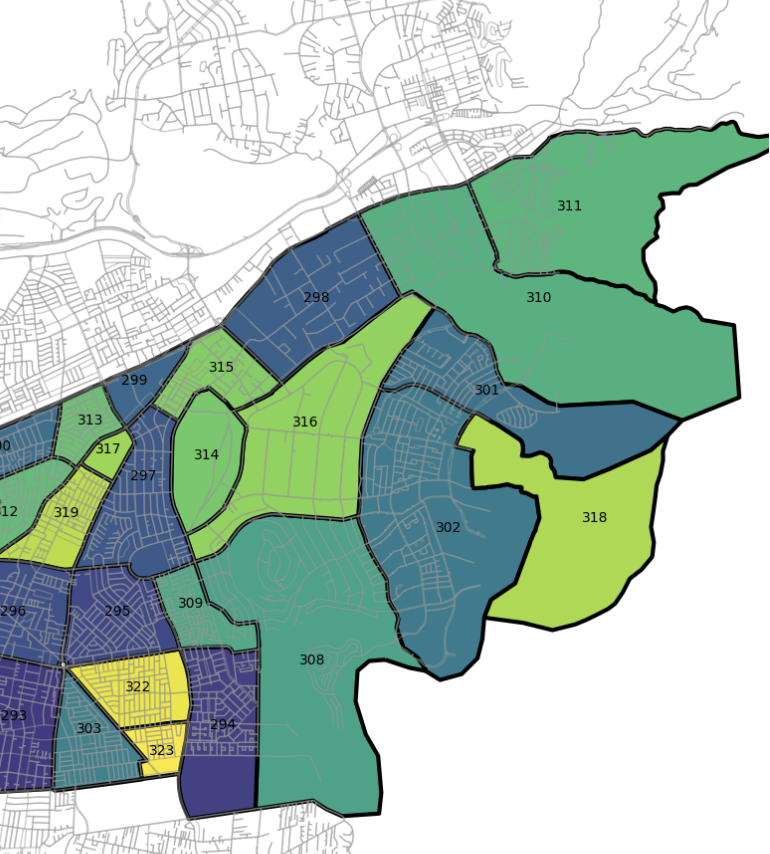
\includegraphics[width=0.35\linewidth]{san_carlos.png}
  \caption{Zonas de San Carlos de Apoquindo}
  \label{fig:zonas}
\end{figure}

\subsection{Generación de Matriz OD aplicando Costos}

En primera instancia, se utilizó un valor de \(K = 1\) para generar la matriz OD:

\begin{table}[H]
  \centering
  \footnotesize
  \begin{tabular}{c|cccccccccc}    
  \textbf{Zona O\textbackslash D} & \textbf{301} & \textbf{302} & \textbf{308} & \textbf{314} & \textbf{316} & \textbf{318} & \textbf{E1} & \textbf{E2} & \textbf{E3} & \textbf{E4} \\ \hline
  \textbf{301} & 1904 & 1718 & 733 & 156 & 166 & 714 & 10 & 23 & 16 & 2 \\ 
  \textbf{302} & 1126 & 8833 & 960 & 873 & 886 & 1131 & 36 & 46 & 91 & 12 \\ 
  \textbf{308} & 1239 & 2477 & 2543 & 999 & 596 & 413 & 33 & 30 & 134 & 15 \\ 
  \textbf{314} & 2 & 17 & 7 & 18 & 5 & 1 & 0 & 0 & 0 & 0 \\ 
  \textbf{316} & 326 & 2665 & 695 & 774 & 626 & 209 & 25 & 27 & 35 & 6 \\ 
  \textbf{318} & 0 & 0 & 0 & 0 & 0 & 0 & 0 & 0 & 0 & 0 \\ 
  \textbf{E1} & 6 & 33 & 12 & 17 & 8 & 4 & 0 & 0 & 0 & 0 \\ 
  \textbf{E2} & 27 & 85 & 21 & 23 & 17 & 12 & 0 & 0 & 0 & 0 \\ 
  \textbf{E3} & 47 & 402 & 228 & 110 & 51 & 28 & 0 & 0 & 0 & 0 \\ 
  \textbf{E4} & 4 & 28 & 14 & 11 & 5 & 3 & 0 & 0 & 0 & 0 \\ 
  \end{tabular}
  \caption{Matriz OD con K = 1}
  \label{table:M_K1}
\end{table}

Donde los vectores correspondientes son:

\begin{table}[H]
  \centering
  \footnotesize
  \begin{tabular}{c|cccccccccc}    
  \textbf{} & \textbf{301} & \textbf{302} & \textbf{308} & \textbf{314} & \textbf{316} & \textbf{318} & \textbf{E1} & \textbf{E2} & \textbf{E3} & \textbf{E4} \\ \hline
  \textbf{O} & 5442.0 & 13994.0 & 8479.0 & 50.0 & 5388.0 & 0.0 & 80.0 & 185.0 & 866.0 & 65.0 \\ 
  \textbf{D} & 4681.0 & 16258.0 & 5213.0 & 2981.0 & 2360.0 & 2515.0 & 104.0 & 126.0 & 276.0 & 35.0 \\ 
  \end{tabular}
  \caption{Vectores Matriz OD con K = 1}
  \label{table:data_matrix}
\end{table}

El error observado es de 1501465.33.

\subsubsection{Calibración de K}

Finalmente, se determinó que el error se minimizaba con un valor de \(K = -2.339\), aun así, siguiendo lo estipulado por la pauta, se utilizó el menor valor posible mayor a 0, es decir, 0.001, lo cual da la siguiente matriz:

\begin{table}[H]
  \centering
  \footnotesize
  \begin{tabular}{c|cccccccccc}    
  \textbf{Zona O\textbackslash D} & \textbf{301} & \textbf{302} & \textbf{308} & \textbf{314} & \textbf{316} & \textbf{318} & \textbf{E1} & \textbf{E2} & \textbf{E3} & \textbf{E4} \\ \hline
  \textbf{301} & 512 & 1705 & 602 & 260 & 197 & 295 & 50 & 62 & 78 & 21 \\ 
  \textbf{302} & 1117 & 6211 & 1385 & 1040 & 742 & 801 & 179 & 150 & 362 & 93 \\ 
  \textbf{308} & 1018 & 3573 & 1707 & 970 & 579 & 512 & 158 & 107 & 434 & 108 \\ 
  \textbf{314} & 3 & 20 & 7 & 6 & 3 & 2 & 1 & 1 & 2 & 1 \\ 
  \textbf{316} & 389 & 2231 & 675 & 520 & 333 & 244 & 103 & 75 & 138 & 44 \\ 
  \textbf{318} & 0 & 0 & 0 & 0 & 0 & 0 & 0 & 0 & 0 & 0 \\ 
  \textbf{E1} & 30 & 165 & 56 & 64 & 31 & 18 & 0 & 0 & 0 & 0 \\ 
  \textbf{E2} & 76 & 279 & 77 & 70 & 46 & 38 & 0 & 0 & 0 & 0 \\ 
  \textbf{E3} & 223 & 1591 & 739 & 399 & 201 & 133 & 0 & 0 & 0 & 0 \\ 
  \textbf{E4} & 33 & 221 & 100 & 74 & 35 & 22 & 0 & 0 & 0 & 0 \\ 
  \end{tabular}
  \caption{Matriz OD con K calibrado a 0.001}
  \label{table:M_K2}
\end{table}

Donde los vectores correspondientes son: 

\begin{table}[H]
  \centering
  \footnotesize
  \begin{tabular}{c|cccccccccc}    
  \textbf{} & \textbf{301} & \textbf{302} & \textbf{308} & \textbf{314} & \textbf{316} & \textbf{318} & \textbf{E1} & \textbf{E2} & \textbf{E3} & \textbf{E4} \\ \hline
  \textbf{O} & 3782.0 & 12080.0 & 9166.0 & 46.0 & 4752.0 & 0.0 & 364.0 & 586.0 & 3286.0 & 485.0 \\ 
  \textbf{D} & 3401.0 & 15996.0 & 5348.0 & 3403.0 & 2167.0 & 2065.0 & 491.0 & 395.0 & 1014.0 & 267.0 \\ 
  \end{tabular}
  \caption{Vectores Matriz OD con K calibrado a 0.001}
  \label{table:data_matrix}
\end{table}

El error observado es de 996057.27.

\subsection{Aplicación del Método Furness en la Matriz OD con K Optimizado}

Posteriormente, se aplicó el método de Furness a esta última matriz OD, según los vectores entregados para 2024:

\begin{table}[H]
  \centering
  \footnotesize
  \begin{tabular}{c|cccccccccc}    
  \textbf{} & \textbf{301} & \textbf{302} & \textbf{308} & \textbf{314} & \textbf{316} & \textbf{318} & \textbf{E1} & \textbf{E2} & \textbf{E3} & \textbf{E4} \\ \hline
  \textbf{O} & 7737 & 15089 & 6632 & 2308 & 4425 & 2784 & 2464 & 899 & 3042 & 5746 \\ 
  \textbf{D} & 1744 & 5736 & 4995 & 20 & 2301 & 1 & 3191 & 2337 & 15240 & 15561 \\ 
  \end{tabular}
  \caption{Vectores 2024}
  \label{table:V_2024}
\end{table}

Obteniendo los siguientes resultados:

\begin{table}[H]
  \centering
  \footnotesize
  \begin{tabular}{c|cccccccccc}    
  \textbf{Zona O\textbackslash D} & \textbf{301} & \textbf{302} & \textbf{308} & \textbf{314} & \textbf{316} & \textbf{318} & \textbf{E1} & \textbf{E2} & \textbf{E3} & \textbf{E4} \\ \hline
  \textbf{301} & 120 & 225 & 172 & 0 & 68 & 0 & 775 & 779 & 3029 & 3013 \\ 
  \textbf{302} & 123 & 387 & 187 & 1 & 121 & 0 & 1310 & 890 & 6638 & 6301 \\ 
  \textbf{308} & 44 & 88 & 91 & 0 & 38 & 0 & 457 & 251 & 3149 & 2895 \\ 
  \textbf{314} & 7 & 25 & 19 & 0 & 10 & 0 & 148 & 120 & 742 & 1370 \\ 
  \textbf{316} & 29 & 92 & 61 & 0 & 36 & 0 & 501 & 296 & 1683 & 1982 \\ 
  \textbf{318} & 0 & 0 & 0 & 0 & 0 & 0 & 0 & 0 & 0 & 0 \\ 
  \textbf{E1} & 328 & 1019 & 750 & 5 & 503 & 0 & 0 & 0 & 0 & 0 \\ 
  \textbf{E2} & 182 & 378 & 226 & 1 & 164 & 0 & 0 & 0 & 0 & 0 \\ 
  \textbf{E3} & 308 & 1242 & 1251 & 4 & 412 & 0 & 0 & 0 & 0 & 0 \\ 
  \textbf{E4} & 603 & 2279 & 2237 & 9 & 948 & 0 & 0 & 0 & 0 & 0 \\ 
  \end{tabular}
  \caption{Matriz OD 2024}
  \label{table:M_2024}
\end{table}

Donde los vectores correspondientes son:

\begin{table}[H]
  \centering
  \footnotesize
  \begin{tabular}{c|cccccccccc}    
  \textbf{} & \textbf{301} & \textbf{302} & \textbf{308} & \textbf{314} & \textbf{316} & \textbf{318} & \textbf{E1} & \textbf{E2} & \textbf{E3} & \textbf{E4} \\ \hline
  \textbf{O} & 8181.0 & 15958.0 & 7013.0 & 2441.0 & 4680.0 & 0.0 & 2605.0 & 951.0 & 3217.0 & 6076.0 \\ 
  \textbf{D} & 1744.0 & 5735.0 & 4994.0 & 20.0 & 2300.0 & 0.0 & 3191.0 & 2336.0 & 15241.0 & 15561.0 \\ 
  \end{tabular}
  \caption{Vectores Matriz OD 2024}
  \label{table:data_matrix}
\end{table}

\newpage
\section{Análisis de Resultados}

En primer lugar, y analizando los datos entregados por el enunciado, se puede apreciar que la matriz del año 2012 (\ref{table:M_2012}) presenta una mayor tasa de flujo hacia las zonas universitarias (D = 302), lo cual hace sentido y se corrobora con los datos obtenidos a partir de la primera tarea.
\\ \\
Posteriormente, se generó la matriz OD con K = 1 (\ref{table:M_K1}), donde se observa una correlación con los datos presentados por la matriz del 2012 (\ref{table:M_2012}). Luego se logró minimizar el error cuadrático medio, observando simplemente una disminución en la cantidad de viajes, manteniendo las proporciones.
\\ \\
Finalmente, la matriz OD del 2024 (\ref{table:M_2024}) presenta una proporción totalmente diferente en los datos, donde se observa una disminución del flujo hacia las zonas universitarias, y un aumento en las zonas residenciales. Esto se debe a que los vectores entregados como insumo por el enunciado (\ref{table:V_2024}) indicaban tal cambio en su propia estructura. Aunque esto no tiene una correlación con la realidad, fueron los datos presentados por el enunciado, por lo tanto, se generó el análisis respondiendo a la incógnita del porqué de tal cambio.

\section{Conclusiones}

En conclusión, se lograron todos los objetivos propuestos al inicio del presente informe, logrando así generar una matriz OD actualizada según una matriz de años anteriores y otro tipo de datos como insumo.
\\ \\
En particular, se logró generar un modelo que, a partir de cualquier matriz OD y una matriz de costos, pudiera generar la matriz OD correspondiente, optimizar el valor de K minimizando el error cuadrático medio, y finalmente, actualizar esa matriz al año correspondiente según los vectores OD de dicho período.
\\ \\
Finalmente, se logró dar una correcta explicación a todos los resultados obtenidos, de esta manera, considerando todo lo anteriormente expuesto, se puede considerar la práctica como exitosa.

\newpage
\section{Anexos}
\subsection{Matriz de Costos Asociados}

\begin{table}[H]
  \centering
  \footnotesize
  \begin{tabular}{c|cccccccccc}    
  \textbf{Zona O\textbackslash D} & \textbf{301} & \textbf{302} & \textbf{308} & \textbf{314} & \textbf{316} & \textbf{318} & \textbf{E1} & \textbf{E2} & \textbf{E3} & \textbf{E4} \\ \hline
  \textbf{301} & 0.5 & 1.85 & 1.53 & 3.11 & 2.22 & 0.77 & 9.71 & 5.15 & 8.85 & 16.01 \\ 
  \textbf{302} & 1.85 & 1.31 & 2.69 & 2.22 & 1.56 & 1.32 & 9.23 & 6.13 & 7.39 & 14.78 \\ 
  \textbf{308} & 1.53 & 2.69 & 1.25 & 1.81 & 1.81 & 2.31 & 9.02 & 6.74 & 6.05 & 13.56 \\ 
  \textbf{314} & 3.11 & 2.22 & 1.81 & 0.65 & 1.25 & 2.95 & 7.04 & 5.55 & 6.8 & 13.12 \\ 
  \textbf{316} & 2.22 & 1.56 & 1.81 & 1.25 & 0.99 & 2.18 & 7.74 & 5.18 & 7.43 & 14.04 \\ 
  \textbf{318} & 0.77 & 1.32 & 2.31 & 2.95 & 2.18 & 0.5 & 9.78 & 5.97 & 9.01 & 15.82 \\ 
  \textbf{E1} & 9.71 & 9.23 & 9.02 & 7.04 & 7.74 & 9.78 & $\infty$ & $\infty$ & $\infty$ & $\infty$ \\ 
  \textbf{E2} & 5.15 & 6.13 & 6.74 & 5.55 & 5.18 & 5.97 & $\infty$ & $\infty$ & $\infty$ & $\infty$ \\ 
  \textbf{E3} & 8.85 & 7.39 & 6.05 & 6.8 & 7.43 & 9.01 & $\infty$ & $\infty$ & $\infty$ & $\infty$ \\ 
  \textbf{E4} & 16.01 & 14.78 & 13.56 & 13.12 & 14.04 & 15.82 & $\infty$ & $\infty$ & $\infty$ & $\infty$ \\ 
  \end{tabular}
  \caption{Matriz OD 2012 Actualizada}
  \label{table:M_2012_actualizada}
\end{table}

\newpage
\subsection{Furness}

La función utilizada de Furness fue una adaptación de la entregada por el enunciado:

\begin{lstlisting}[language=Python]
  def furness(t, O, D, tol=1e-6, maxit=10000):
    k = len(O)
    O = np.array(O)[:, np.newaxis].astype(float)
    D = np.array(D).astype(float)
    t = np.array(t)
    ai = np.ones((k, 1))
    bj = np.ones((1, k))
    iters = 0
    
    # Añadir un pequeño valor epsilon para evitar divisiones por cero
    epsilon = 1e-10

    while iters < maxit:
        # Calcular ai, evitando división por cero
        t_sum1 = t.sum(axis=1)[:, np.newaxis] + epsilon  
        # Suma de filas con epsilon
        ai = O / t_sum1
        
        # Actualizar t con ai
        t = t * np.dot(ai, np.ones((1, k)))
        
        # Calcular bj, evitando división por cero
        t_sum0 = t.sum(axis=0) + epsilon  
        # Suma de columnas con epsilon
        bj = D / t_sum0
        
        # Actualizar t con bj
        t = t * np.dot(np.ones((k, 1)), bj[np.newaxis, :])
        
        # Verificar convergencia
        if np.max(abs(t_sum1.flatten() / O.flatten() - 1)) < tol:
            break

        iters += 1
    t_rounded = np.rint(t)
    return t_rounded
\end{lstlisting}

%\newpage
%\bibliography{referencias}  % Nombre del archivo .bib

\end{document}
